\chapter{Application overview}
\label{ch:applicationoverview}
\markboth{Application overview}{}

\begin{flushright}
	{\smaller
		\textit{I do not fear computers. \\ I fear the lack of them.}\\
		--  Isaac Asimov}
\end{flushright}
In this Chapter an overview of the \gls{acr:Adopt} software, and its reference library \gls{acr:Jpad} will be presented.
\gls{acr:Adopt} is a Java-based desktop application developed at the University of Naples Federico II, conceived as a fast, reliable and user friendly computational aid for aircraft designers in the conceptual and preliminary design phases. The ultimate goal of such a tool is to perform a parametric, multi-disciplinary analysis of an aircraft and then search for an optimized configuration. The search domain boundaries are usually defined by the user through a set of specifyed parameters. An important design requirement of  \gls{acr:Adopt} is related to its interoperability with other engineering analysis tools. In fact, the application can be easily integrated into a comprehensive aircraft optimization cycle. This is made possible because  \gls{acr:Adopt} can be launched both in \gls{acr:gui} and command line mode. Much care has been given to input/output and configuration files to increase the possible uses of the software.

\begin{figure}[H]
	\centering
	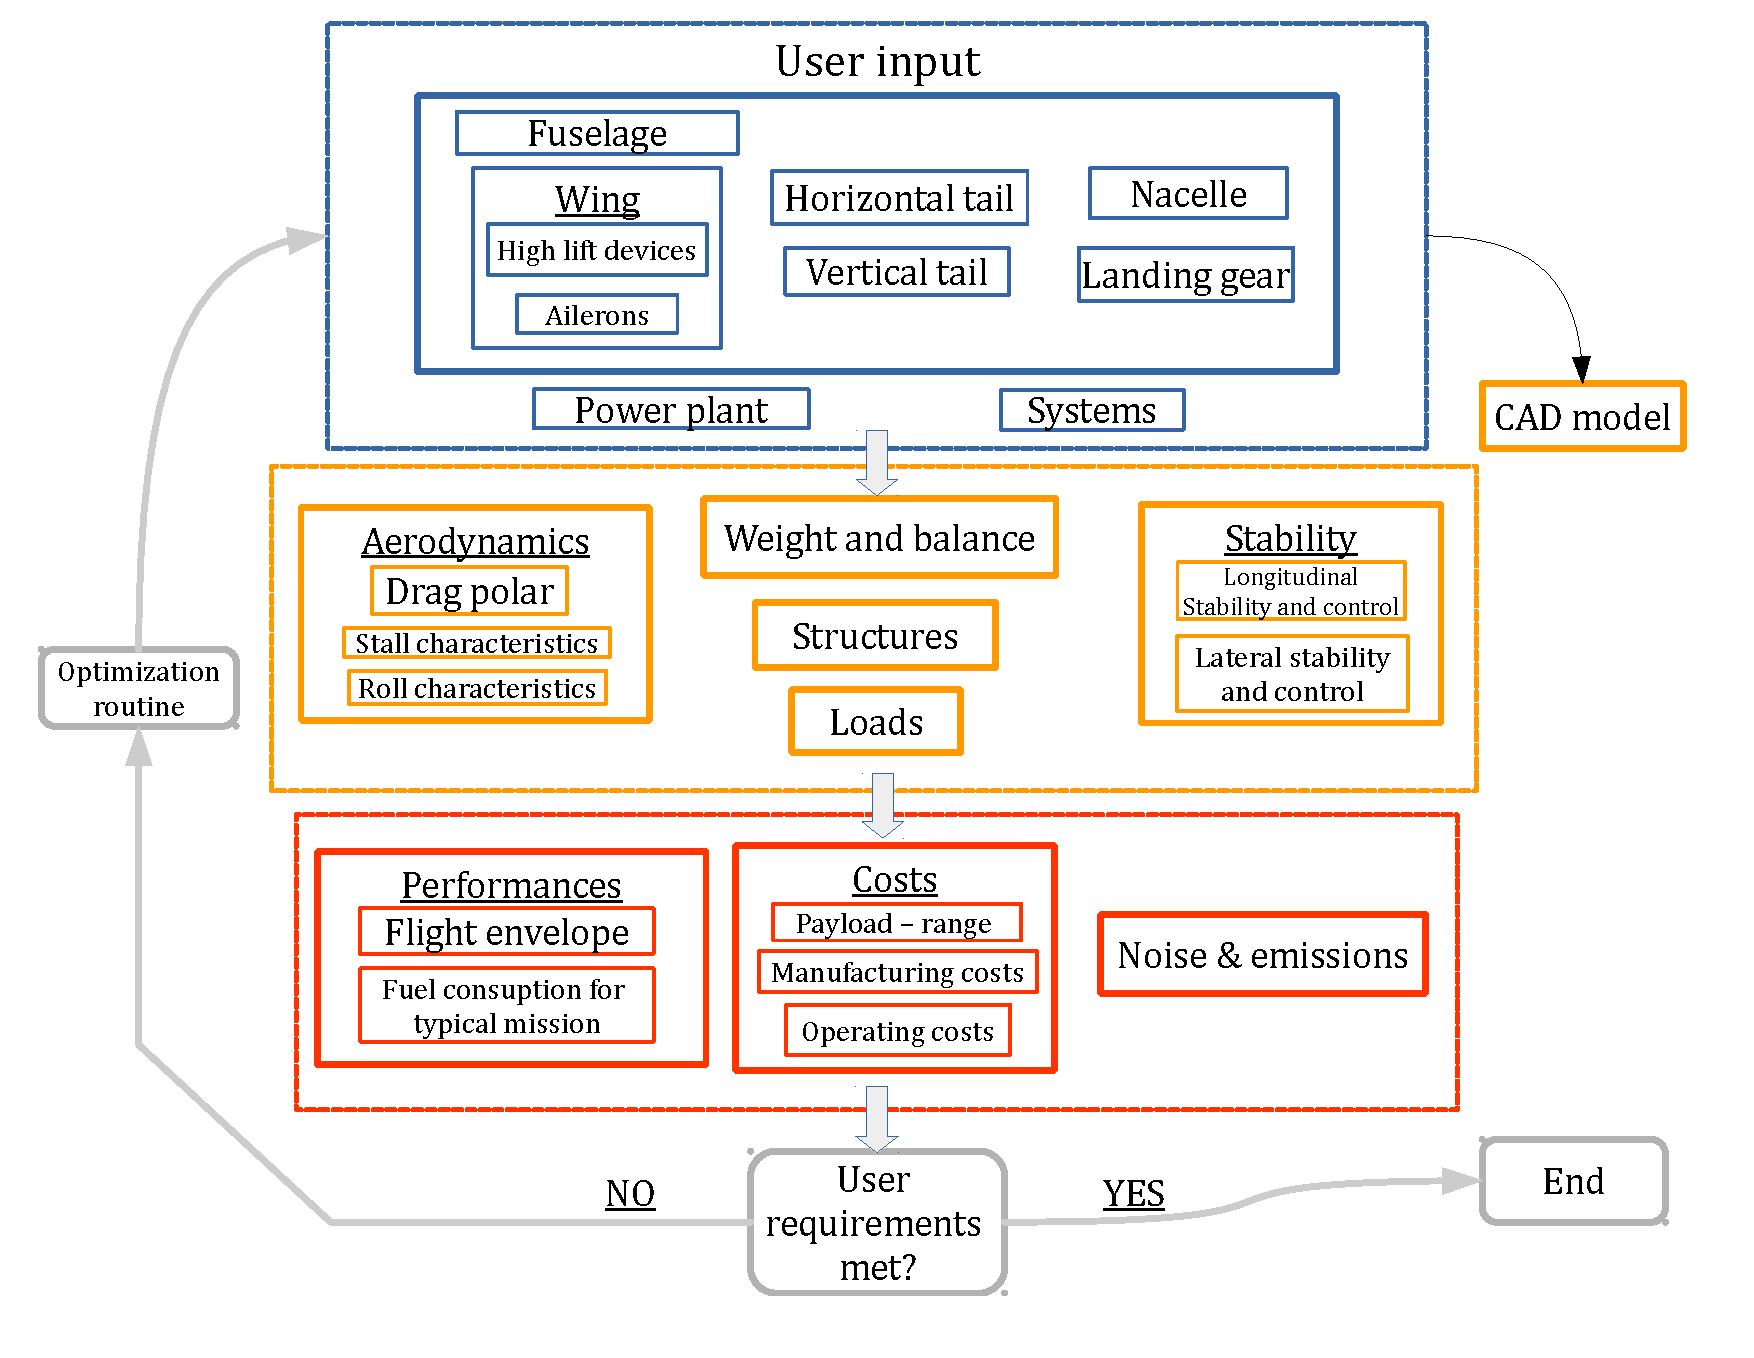
\includegraphics[height = 8.6cm ]{Immagini/flowchart3}
	\caption{Software calculation modules.}
	\label{fig:guiStart}
\end{figure}

\section{Software architecture}

\gls{acr:Jpad} library is actually divided into three package: JPADConfigs, JPADCore and JPADSandbox.  Each package is organized in several classes or more package in order to have a clear and simple classification. The possibility to place similar classes in the same package has been extensively exploited for the same reasons, see section A.2.   The source code has been extensively commented following Javadoc practices. This enabled us to automatically generate documentation using Doxygen \cite{doxgen}

\begin{figure}[H]
	\centering
	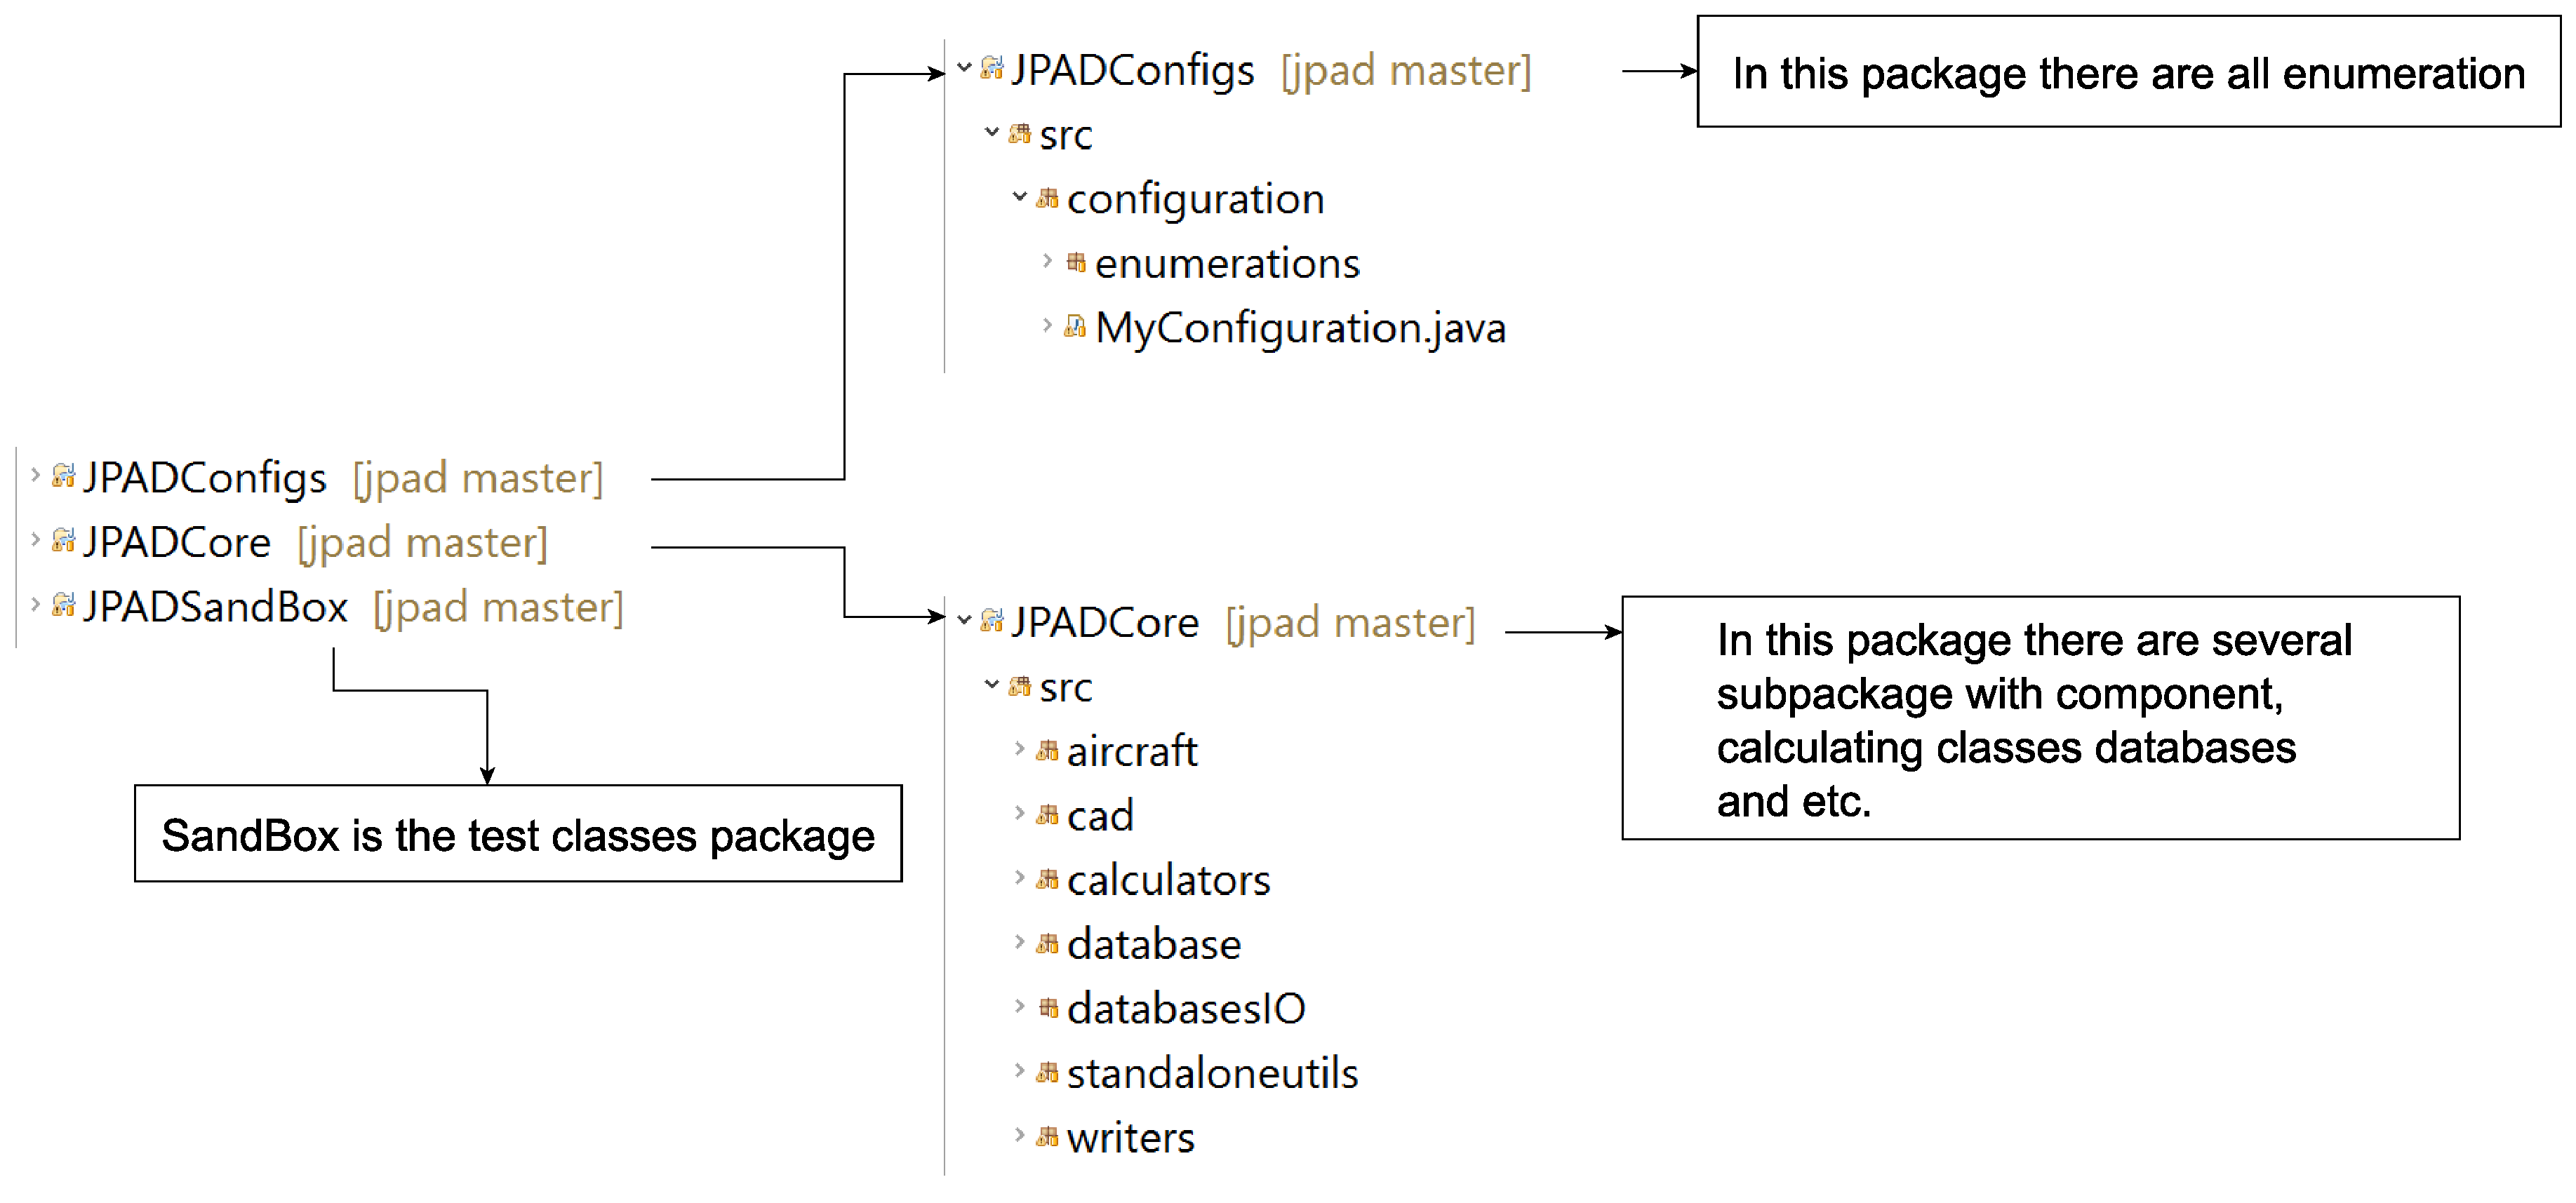
\includegraphics[height = 7.6cm ]{Immagini/organization}
	\caption{Software package division.}
	\label{fig:sw}
\end{figure}
 
 The main package of \gls{acr:Jpad} library is JPADCore where there are all aircraft component, the managers of calculator and  its computers classes. In the following subsection will explained the main features of JPADCore.\\
 JPADCore contains the following sub-packages:
 \begin{enumerate}
 \item \texttt{aircraft} $\rightarrow$ This package contains all aircraft's component classes, their calculators and the related managers and also the operating condition's class.
 \item \texttt{cad} $\rightarrow$  This package contains everything concerning the creation of CAD model.
 \item \texttt{calculators} $\rightarrow$ In this package there are the classes, divided in package by type of analysis, whose methods implement the calculation formulas.
 \item \texttt{database} $\rightarrow$ This package contains the classes that manage the database .h5 whose data are useful for the analysis. 
 \item \texttt{standaloneutils} $\rightarrow$ In this package there are several calculation classes with mathematical tools to support the analysis.
 \item \texttt{writers} $\rightarrow$ this class is in charge of writing files.
 \end{enumerate}
 
 \noindent \\
 Following will be explained the main features of the fundamental packages.
 
 \subsection{\texttt{Aircraft }package}
 Each component (e.g., the fuselage, the wing, the engine) is therefore defined in its own class. In the aircraft package there are other sub-package for components. In each of these there are a class for the object definition and a manager for the analysis. These manager classes uses the utilities located in the calculator package. \\
 The sub-package in the \texttt{aircraft} package are the following:
 
 \begin{itemize}
 \item \texttt{Auxiliary} that manages the airfoils
 \item  \texttt{Component} that contains the \texttt{aircraft} class, the aircraft components packages (fuselage, lifting surfaces, nacelles, power plant, fuel tank, landing gear, systems) and, inside them, their manager analysis classes used to call related analysis methods. 
 \item \texttt{OperatingConditions} 
 \end{itemize}

The main aircraft components are organised as follows: \\ 

Basic data for describing the {\bfseries fuselage} are contained in the \texttt{fuselage} class. This holds all the fuselage overall properties, such as the length, maximum width and maximum height, length ratios between the nose and the tail parts length to the constant section part length, number of decks and so on. Other classes in the package manage the shape of fuselage sections and outlines (which define the fuselage shape in the xz and xy planes) and aerodynamics calculations (Aerodynamics class).\\ \\

The data relating to the {\bfseries lifting surfaces} are contained in the \texttt{liftingSurface } class. Since the lifting surfaces of an aircraft share several characteristics, a single class has beencreated to manage the wing, the horizontal and vertical tail and, eventually, the canard. The lifting surface specific category (that is, wing, horizontal tail etc.) is acknowledged through a \texttt{MyComponentEnum} variable which has to be specified when creating the lifting surface object. By default, a lifting surface has three primary span stations: root ($\eta = 0$), middle and tip ($\eta = 1$). The middle station location is user-defined and is used to represent a change in chord.y/ law; such a change can be due to a lifting surface kink or to the beginning of a tapered part. If the wing is simple tapered the middle station can also be omitted.\\ \\

The data relating to the {\bfseries airfoils} are handled by \texttt{Airfoil} class, that creates for each lifting surface three airfoils, located respectively at $\eta=0$, $\eta=1$ and at middle station. An airfoil object holds:
\begin{enumerate}
	\item the position along the semispan, $\eta$;
	\item twist value relative to root, $\epsilon_g$;
	\item zero lift angle of attack, $\alphazlp$;
	\item angle of attack value at the end of the linear part of $C_l(\alpha)$ curve, $\alphastar$;
	\item stall angle of attack, $\alpha_{stall}$;
	\item lift gradient of the linear part of $C_l(\alpha)$ curve, $\Clalphap$;
	\item minimum drag coefficient, $C_{d,min}$;
	\item lift coefficient at $C_{d,min}$, $C_l@C_{d,min}$;
	\item lift cofficient at the end of linear part;
	\item maximum lift coefficient, $\Clmaxp$
	\item drag polar $K$ factor;
	\item aerodynamic moment coefficient gradient, $C_{m_\alpha}$;
	\item aerodynamic center x coordinate, $x_{ac}$;
	\item aerodynamic moment coefficient with respect to the aerodynamic center, $C_{m_{ac}}$ or $\Cmzerop$;
	\item aerodynamic moment coefficient with respect to the aerodynamic center at stall, $C_{m_{ac},stall}$;
	\item maximum thickness to chord ratio, $t/c_{max}$;
	\item x,z non dimensional coordinates.
\end{enumerate}
At the time of writing all these quantities have to be entered by the user. The \texttt{Airfoil} class provides the \texttt{populateCoordinateList()} method which transforms the non dimensional coordinates provided by the user in order to obtain their actual coordinates, which takes into account of actual chord length, ACRF position, sweep, twist and dihedral.\\ \\

The  {\bfseries power plant} is defined in the package \texttt{PowerPlant} in \texttt{components}. In this package there is the \texttt{engine} class that initializes the data related to the single engine. An other class in the same package, \texttt{powerPlant} creates the parametric model of the power plant using a list of objects creates by \texttt{engine}.


\subsection{\texttt{MyOperatingConditions} class}
As the name suggests, this class contains all the data related to atmosphere conditions (which are currently derived from altitude value using the 1976 ISA model), current speed (Mach number), gravitational acceleration (\SI{9.80665 }{\meter/\second^2}) and sea level pressure (\SI{101325}{\Pa}).

A \texttt{MyOperatingConditions} object can be created regardless of the aircraft configuration as the class is entirely self contained: the aircraft could also be undefined at the time of the object creation. If the user wants to run several analysis at different operating conditions, a \texttt{MyOperatingConditions} instance has to be created for each one.

\subsection{\texttt{CAD} package}

Throughout the development of the application, great care has been given to the making of the CAD model for several reasons:
\begin{itemize}
	\item it enables the user and the user developer to have an immediate feedback about the data provided to the application: if some geometrical parameter is wrong, the CAD model makes it impossible not noticing it;
	\item it allows the user to run a CFD analysis with an external program. The CAD model has been in fact built so that it is ready to be meshed by an external mesher without any further adjustment;
	\item it provides an accurate estimate of the wetted surface of each component.
\end{itemize}

The creation of the CAD model was made possible by the occjava library, whose classes and methods have been used to build each component's model.

 \subsection{\texttt{Calculators} package}
 This package includes all the calculators classes. Calculator classes have been created to evaluate quantities related with more than one component. The calculator classes are the following:
 
 \begin{itemize}
 \item {\texttt{aerodynamics} package}
\item {\texttt{cost} package}
\item {\texttt{geometry} package}
\item {\texttt{performance} package}
\item {\texttt{stability} package}
\end{itemize} 

Each of these package contains calculators classes and concerning methods that implement all mathematical equations. These methods are called by the analysis manager classes that are in the package of relatives components (such as fuselage, lifting surfaces etc.).

\subsection{\texttt{Database} package}
In order to manage a large quantity of data, it has been necessary to read data from graphs available in literature; for such a reason an extensive database has been built over the years by several of my colleagues to digitalize this data in order to exploit it in a computer program. The data has been stored in an hdf5 file.\\
In the \texttt{database} package there are all the classes that manage and reads the .h5 files. To obtain the useful data in JPAD, interpolating functions are used . These functions can be of one, two or three dimensions and read data from graphics that have been digitize previously.

\subsection{\texttt{Writers} package}
 This class is based on the Apache POI library and provides methods which enable the user developer to easily add a sheet to an XLS file, to set the styles of the XLS file and to compare different XLS files.The last function permits to create an XLS file which contains a different aircraft data for each column; in such a way the comparison between two or more aircraft (or,
simply, between slightly different configurations of the same aircraft) is easier and effective.



\section{Graphical User Interface (GUI)}
An extensive work has been done to set up an effective Graphical User interface (GUI) to reduce the time the user has to spend to obtain relevant results. The result presented in this section is the early step of graphical interface, which is currently in development.\\ 

The Java programming language greatly helped to build the GUI: several open source libraries (SWT, JFace) allowed us to build a functional yet pleasant GUI which allows the user to easily change the aircraft’s parameters, to view a 3D model of the defined geometry, to launch a new analysis and view the corresponding results. The current GUI appearance is shown in fig. \ref{fig:guiStart}. It is composed of several items:
\begin{enumerate}
	\item a menu bar (on top), which holds all the available actions divided in sub-categories;
	\item a toolbar (below the menu bar), which holds the most important actions needed to interact with the application. The toolbar, as the menu bar, is always visible to the user;
	\item a project tree (on the left), a key component of the GUI since it provides access to all the components of the aircraft and the analysis results any time during the execution of the application. The project tree appears once an aircraft is created and can be eventually hidden;
	\item a 3D view, which shows the CAD model of the aircraft selected by the user. The CAD model can be updated each time the user wants to check the changes made to the aircraft geometry;
	\item a log message window, placed at the bottom, that tells the user the status of pending operations. This window can be hidden;
	\item a tab folder, which contains all the windows opened using the project tree; these windows can be closed and reopened any time.
\end{enumerate}


\begin{figure}[H]
	\centering
	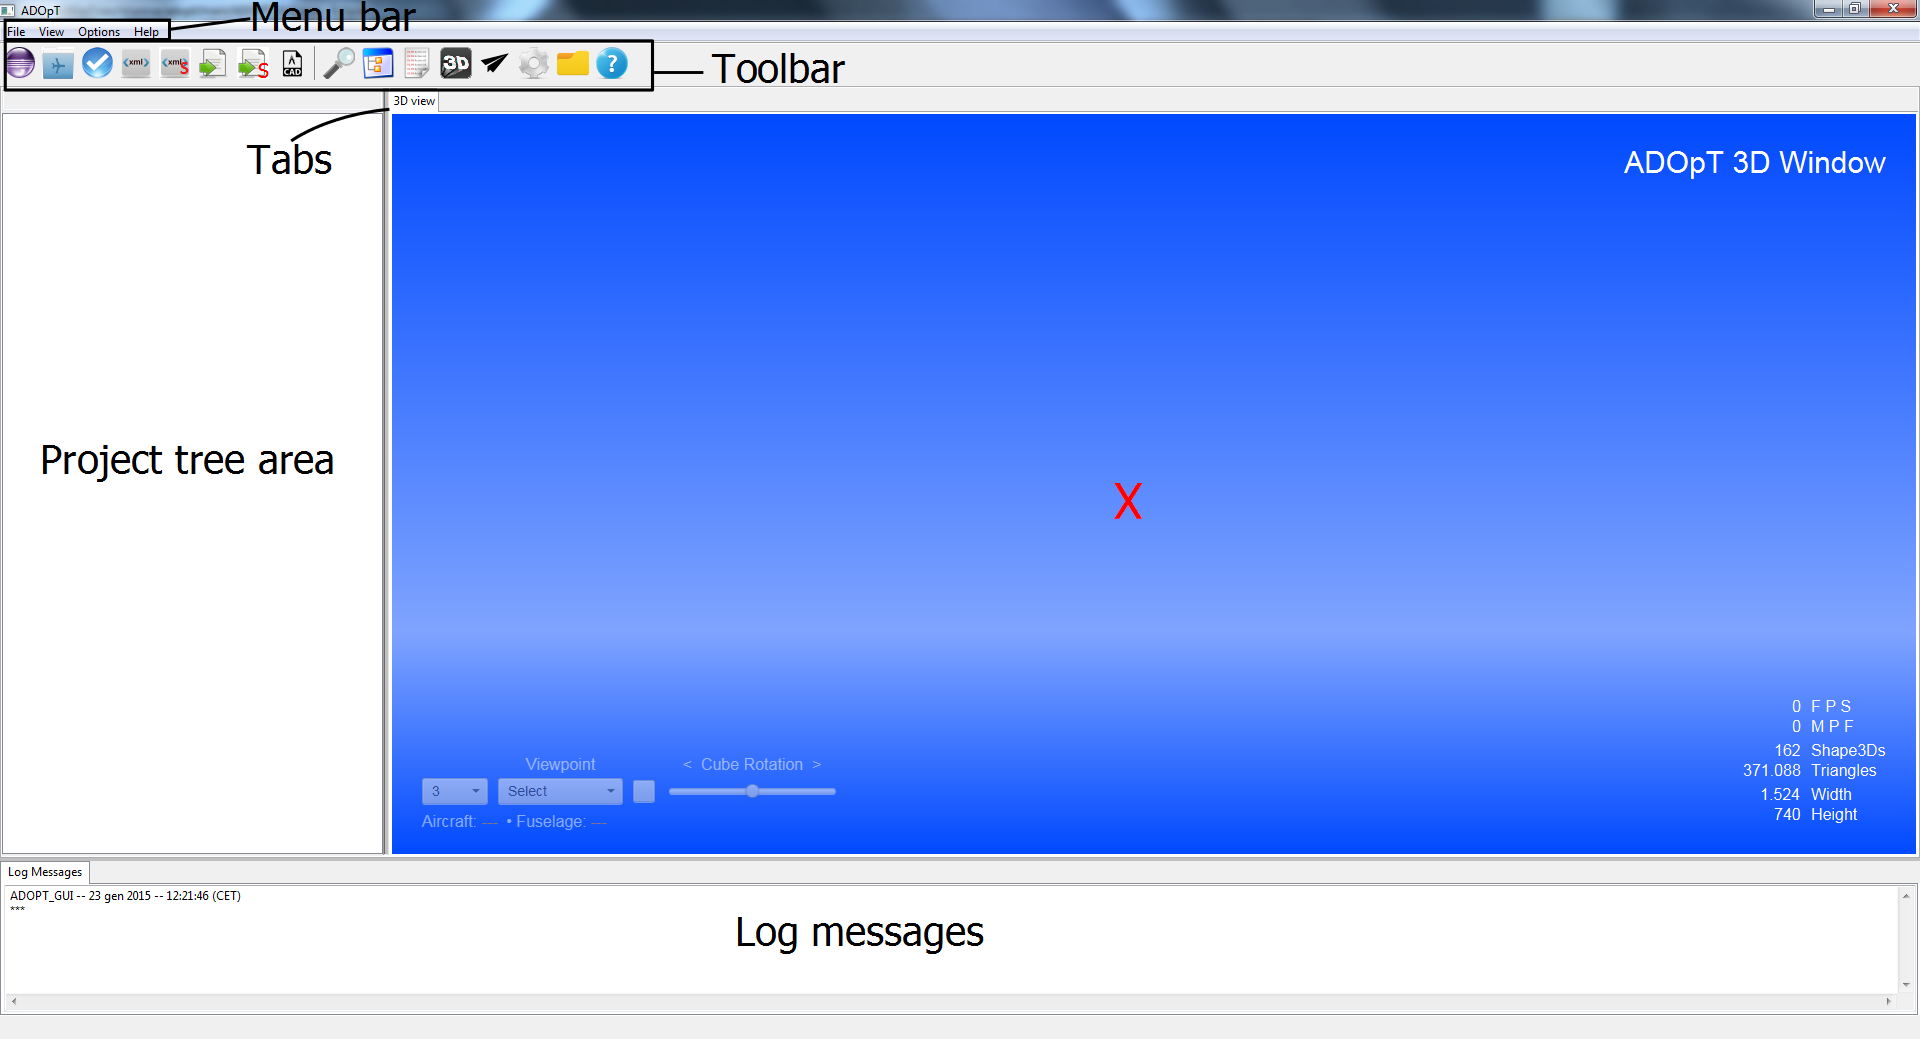
\includegraphics[height = 7cm ]{Immagini/gui/applicationStart.png}
	\caption{The GUI when the application is started.}
	\label{fig:guiStart}
\end{figure}

\subsection{Typical work session}
In developing the application we focused on making the user's typical work session as simple as possible. Few basics steps are required for running an analysis:

\begin{enumerate}
\item create a new aircraft, which we will call A. This can be done using the corresponding button \big(
\includegraphics[scale=0.6]{Immagini/gui/icons/FolderAirplane_32x32.png}\big) in the toolbar, which instantiates the default aircraft
	
\item set the parameters that define the aircraft model using the corresponding window opened using the tree
\begin{figure}[H]
		\centering
		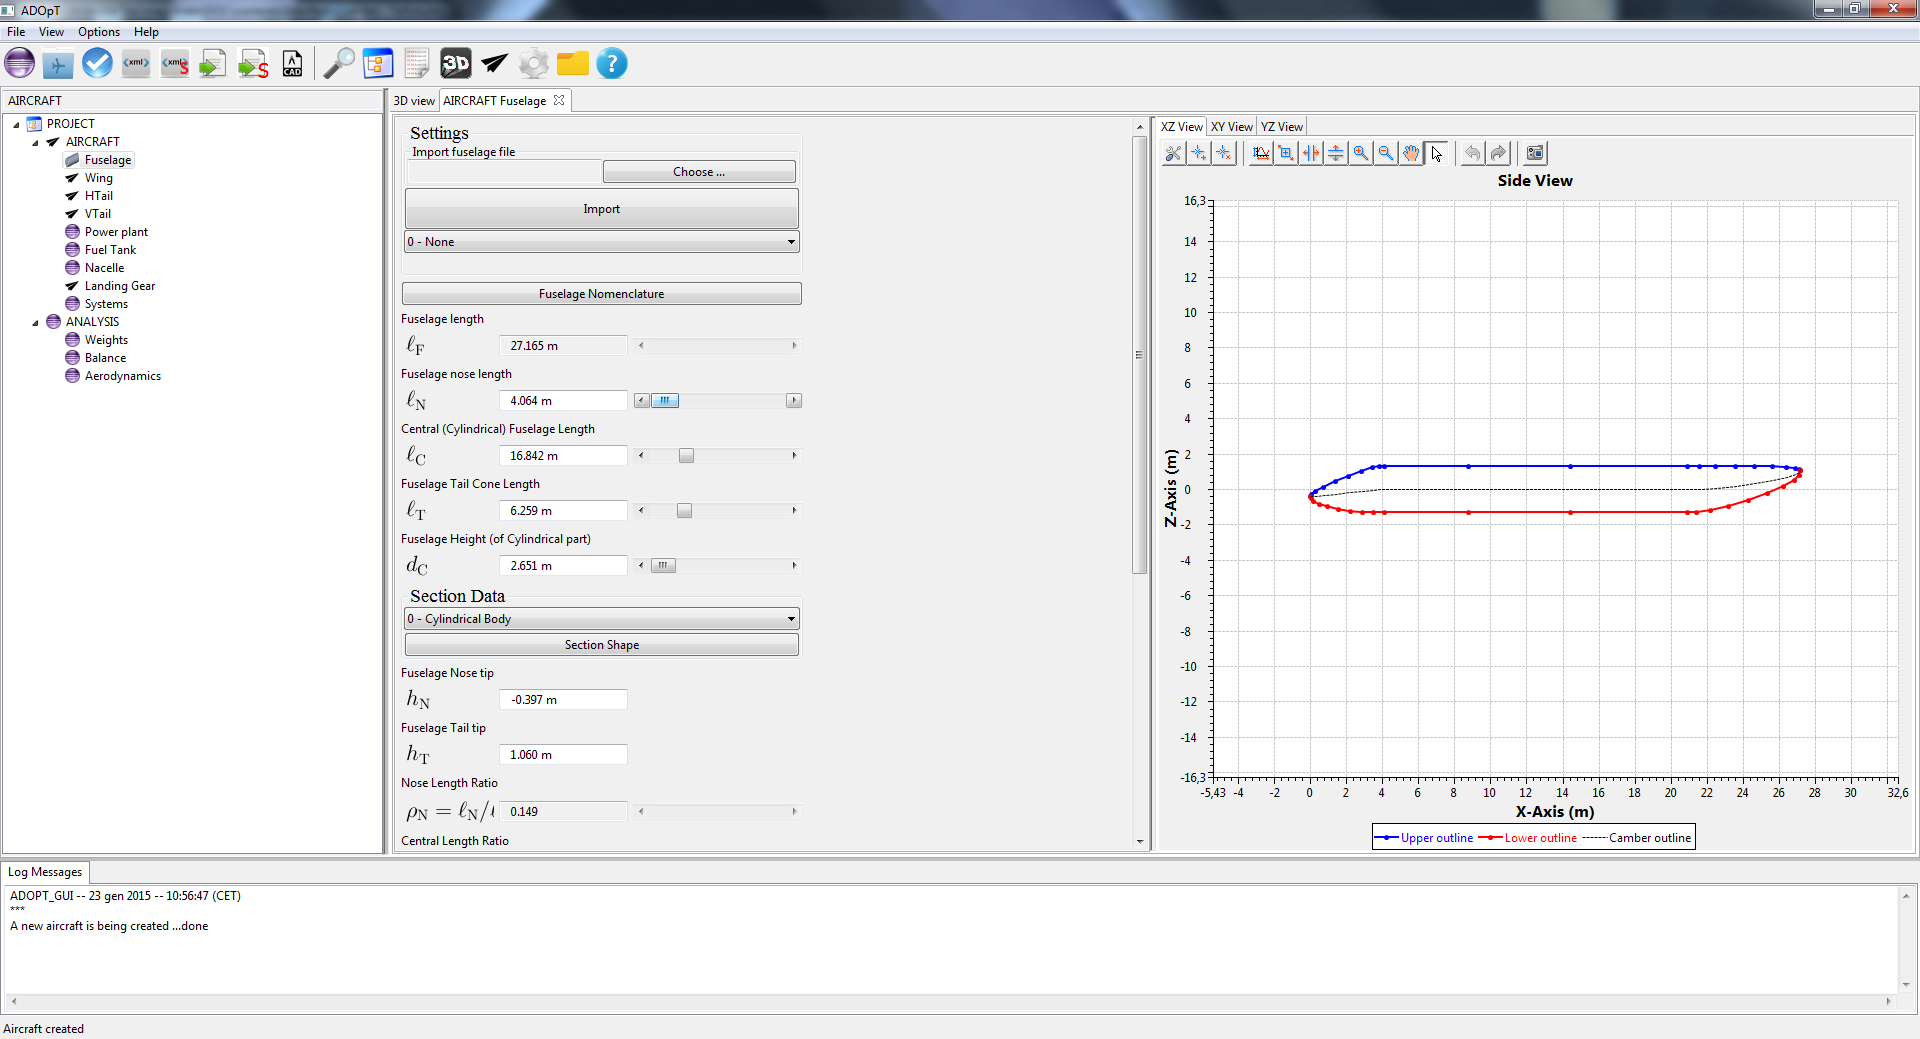
\includegraphics[height = 7cm]{Immagini/gui/changeFusParam.png}
		\caption{The window for changing the fuselage parameters.}
	\end{figure}
\item explore the 3D model \big(
\includegraphics[scale=1.2]{Immagini/gui/icons/3DView_32x32.png}\big) of the aircraft and eventually change some parameters if there is some error
		\begin{figure}[H]
	\centering
		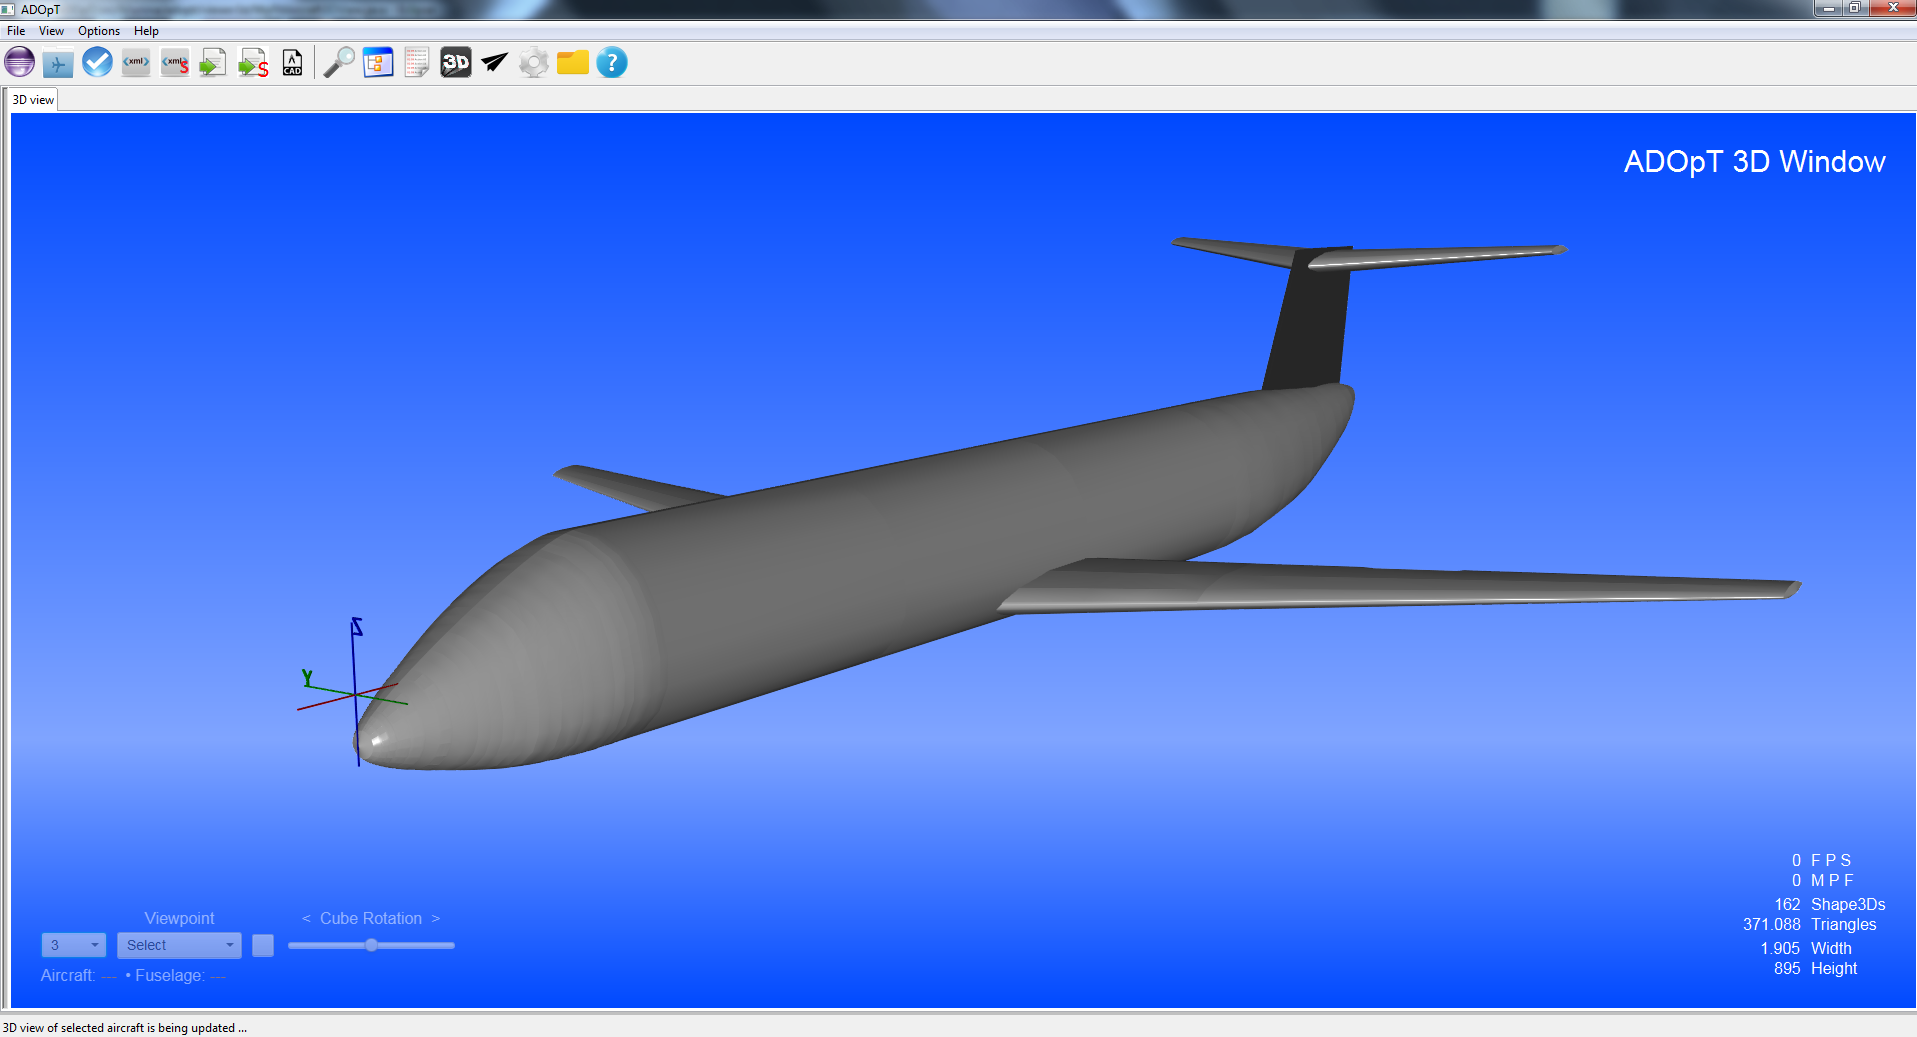
\includegraphics[height =7cm]{Immagini/gui/cad1.png}
		\caption{The aircraft 3D view (log window and project tree hidden).}
	\end{figure}
\item execute a complete analysis \big(
\includegraphics[scale=0.5]{Immagini/gui/icons/analysis_32x32.png}\big) of the aircraft previously defined;

	\item export the analysis results to an XML and/or an XLS file \big(
\includegraphics[scale=0.4]{Immagini/gui/icons/Export_32x32.png}\big);
	
	\item eventually export the CAD model of the aircraft \big(
\includegraphics[scale=1.2]{Immagini/gui/icons/cad_32x32.png}\big);
	\item save the current aircraft to an XML file \big(
\includegraphics[scale=0.4]{Immagini/gui/icons/XML_32x32.png}\big).
\end{enumerate}

	
At this point the user could simply change the current configuration until the analysis results are satisfactory. The application can however help the user in finding such a configuration, since it can hold multiple configurations simultaneously, analyse all of them and compare them side by side. To accomplish this task, once the first aircraft has been created, the user should:

\begin{enumerate}
	\item import the aicraft previously saved or create an entirely new aircraft, which we will call B;
	\item change B parameters and run a new analysis on it;
	\item study the results and eventually change some of the parameters;
	\item save every configuration and the corresponding results to file;
	\item export both aircraft and the corresponding results to an XLS file.
\end{enumerate}
	
	\begin{figure}[H]
	\centering
		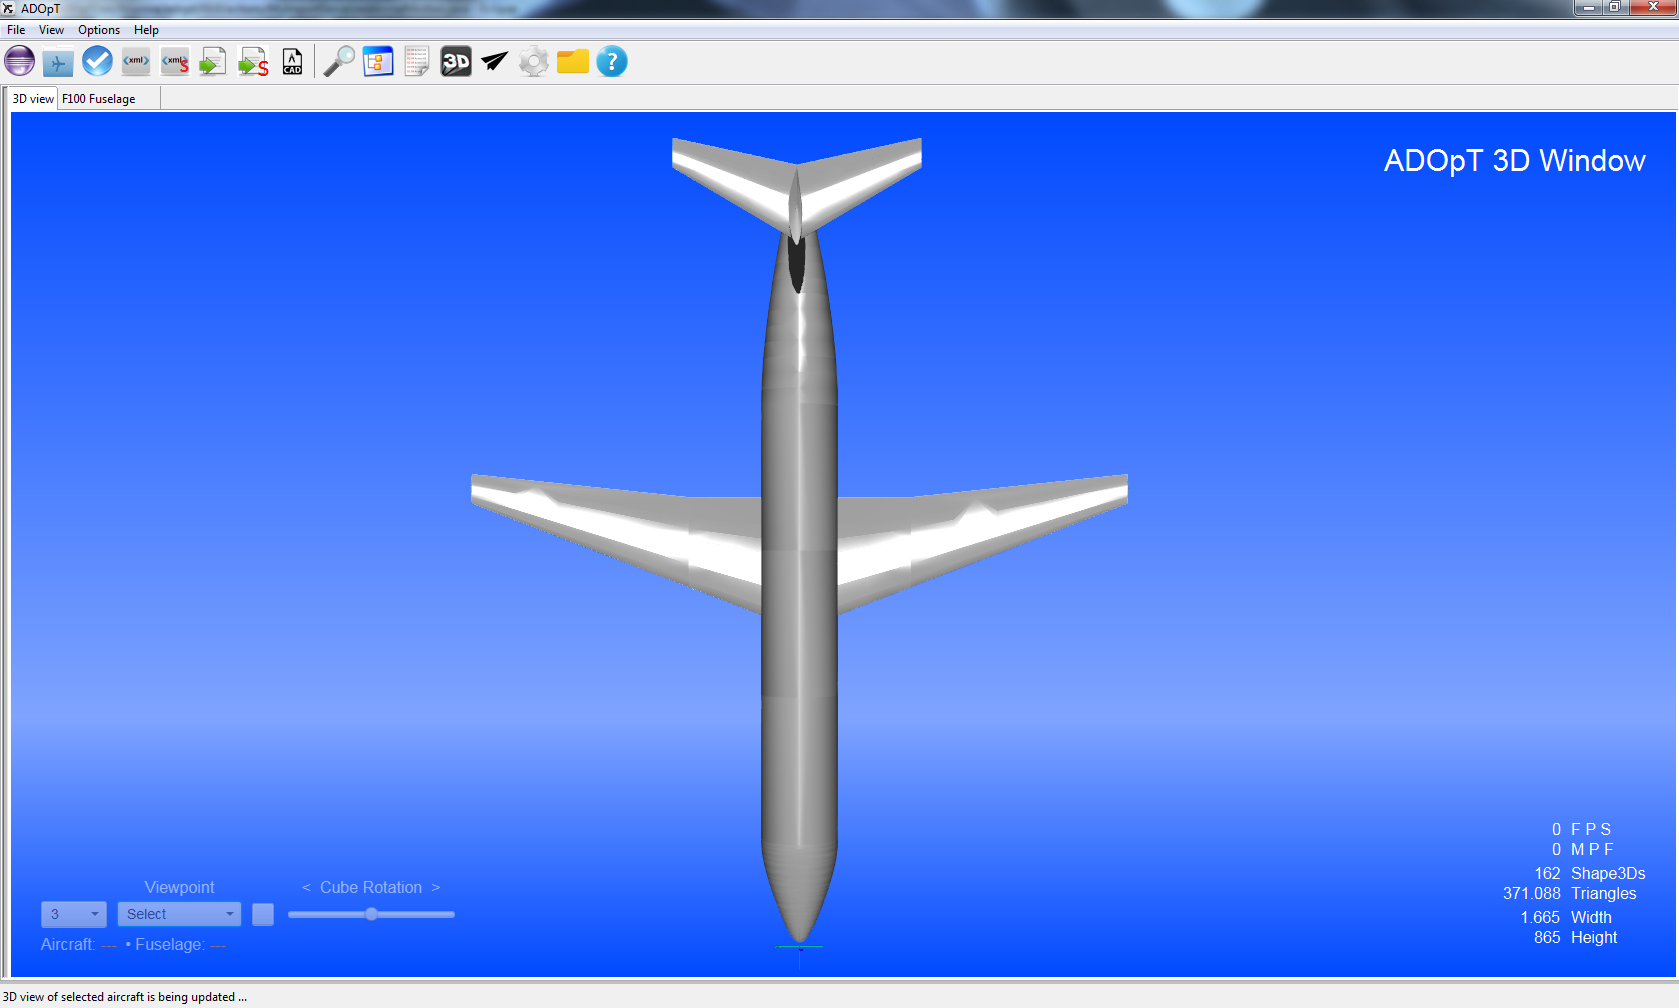
\includegraphics[height =8cm]{Immagini/gui/cad3.png}
		\caption{The aircraft 3D view.}
	\end{figure}		
%

%\begin{figure}[H]
%		\centering
%		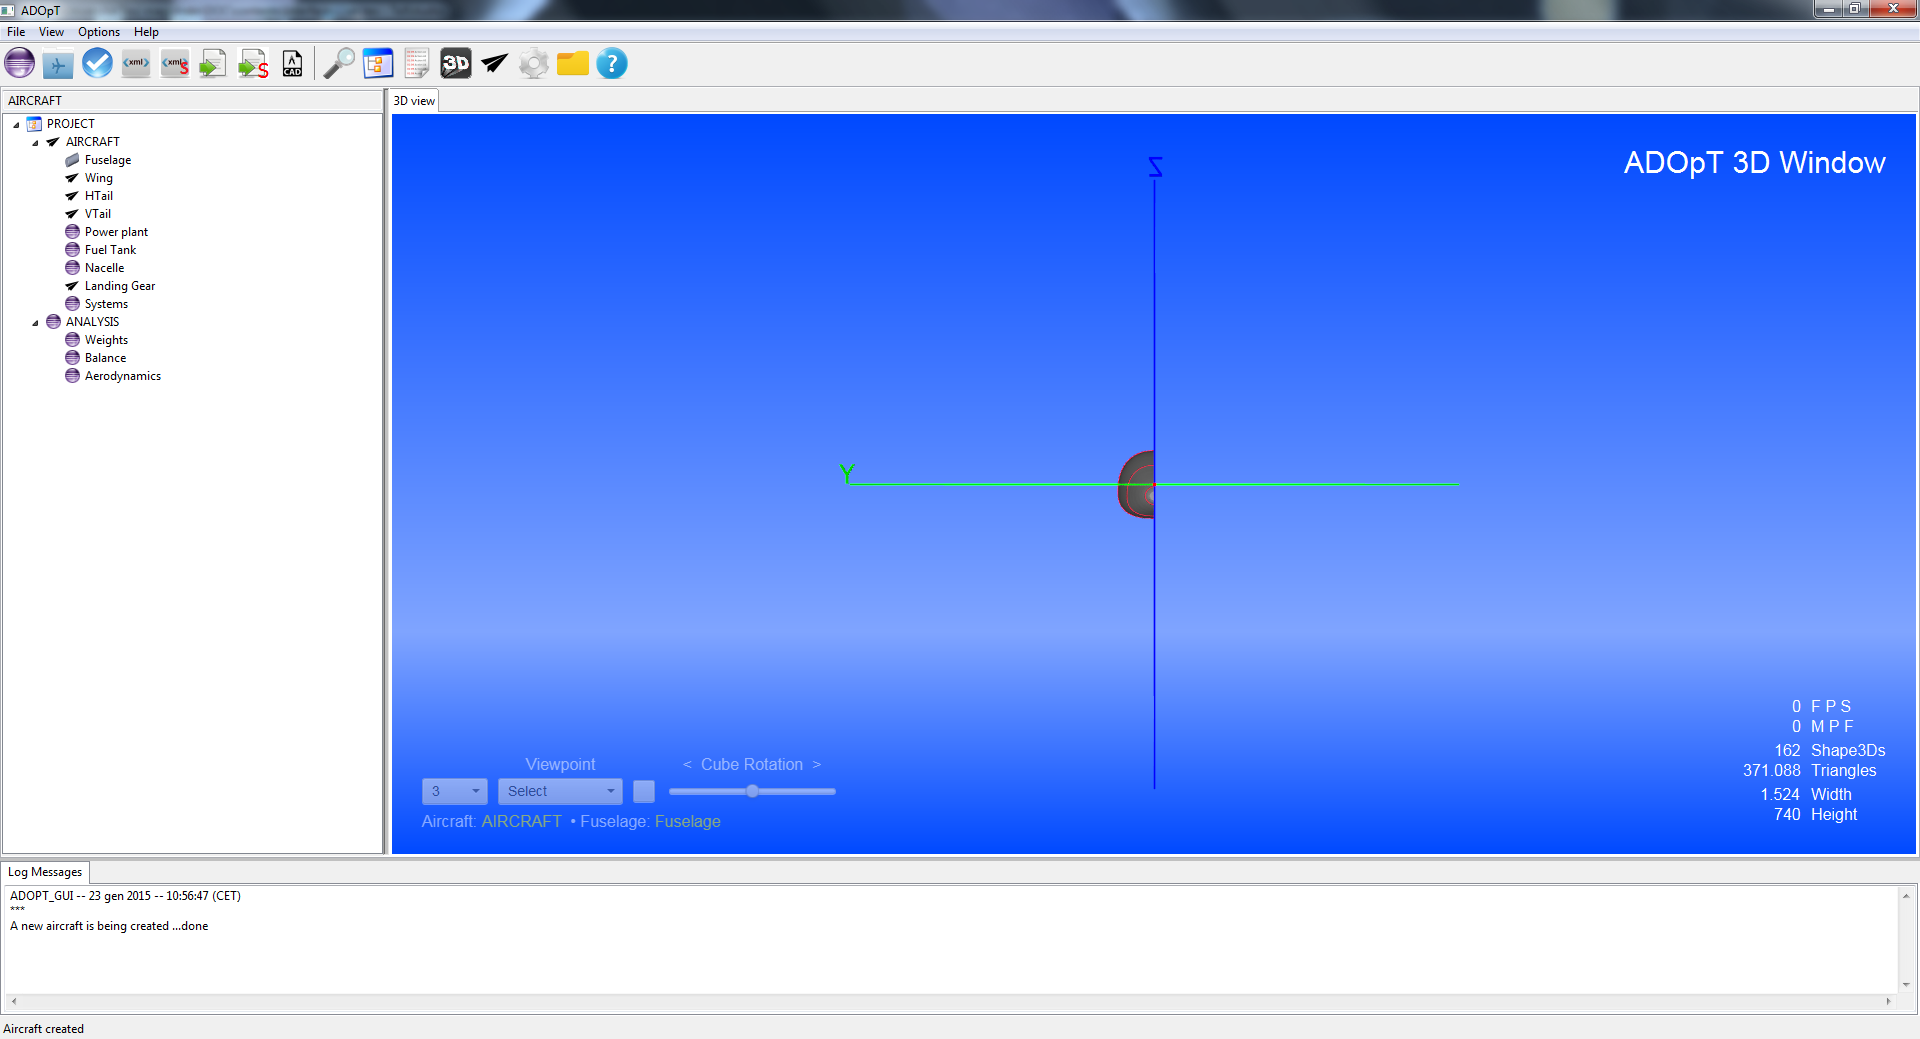
\includegraphics[height = 8cm ]{Immagini/gui/createAircraftDone.png}
%		\caption{The GUI as it appears when an aircraft is created.}
%		\label{fig:guiDescription}
%	\end{figure}


There is no limit to the number of aircraft the application can handle; each aircraft is added to the project tree as shown in fig. \ref{fig:projectTreeMulti} providing access to the corresponding components and analysis.

\begin{figure}[H]
	\centering
	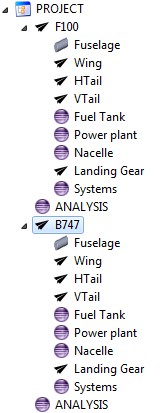
\includegraphics[height=8cm]{Immagini/gui/projectTreeMulti.png}
	\caption{The project tree holding two different aircraft}
	\label{fig:projectTreeMulti}
\end{figure}

\begin{figure}[h]
	\centering
	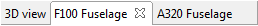
\includegraphics[width=5cm]{Immagini/gui/tabId.png}
	\caption{Same component tab belonging to different aircraft}
	\label{fig:tabId}
\end{figure}



\subsection{CAD modelling}
The application can also be used as a basic parametric \gls{acr:cad} modeler. The capability to change the aircraft parameters using the corresponding controls in the \gls{acr:gui}, coupled with the 3D view, allows the user to change each component shape and dimension, view the updated \gls{acr:cad}model and eventually export it to file once some satisfactory results have been obtained.\\
The creation of the CAD model was made possible by the occjava library, whose classes and methods have been used to build each component’s model. The CAD model can be saved in two different file formats: STEP and BREP; they have proven to take both little memory and to give the best results in terms of geometry representation. The IGES format gave instead mixed results so we preferred to use only the first two.

\begin{figure}[H]
	\centering
		\includegraphics[width=6 cm]{Immagini/gui/CADfuselageTailBAD2.png}
		\caption{A detail of the tail of the fuselage obtained as a unique loft.}
		\label{fig:badTail}
	\end{figure}
	
	\begin{figure}[H]
	\centering
		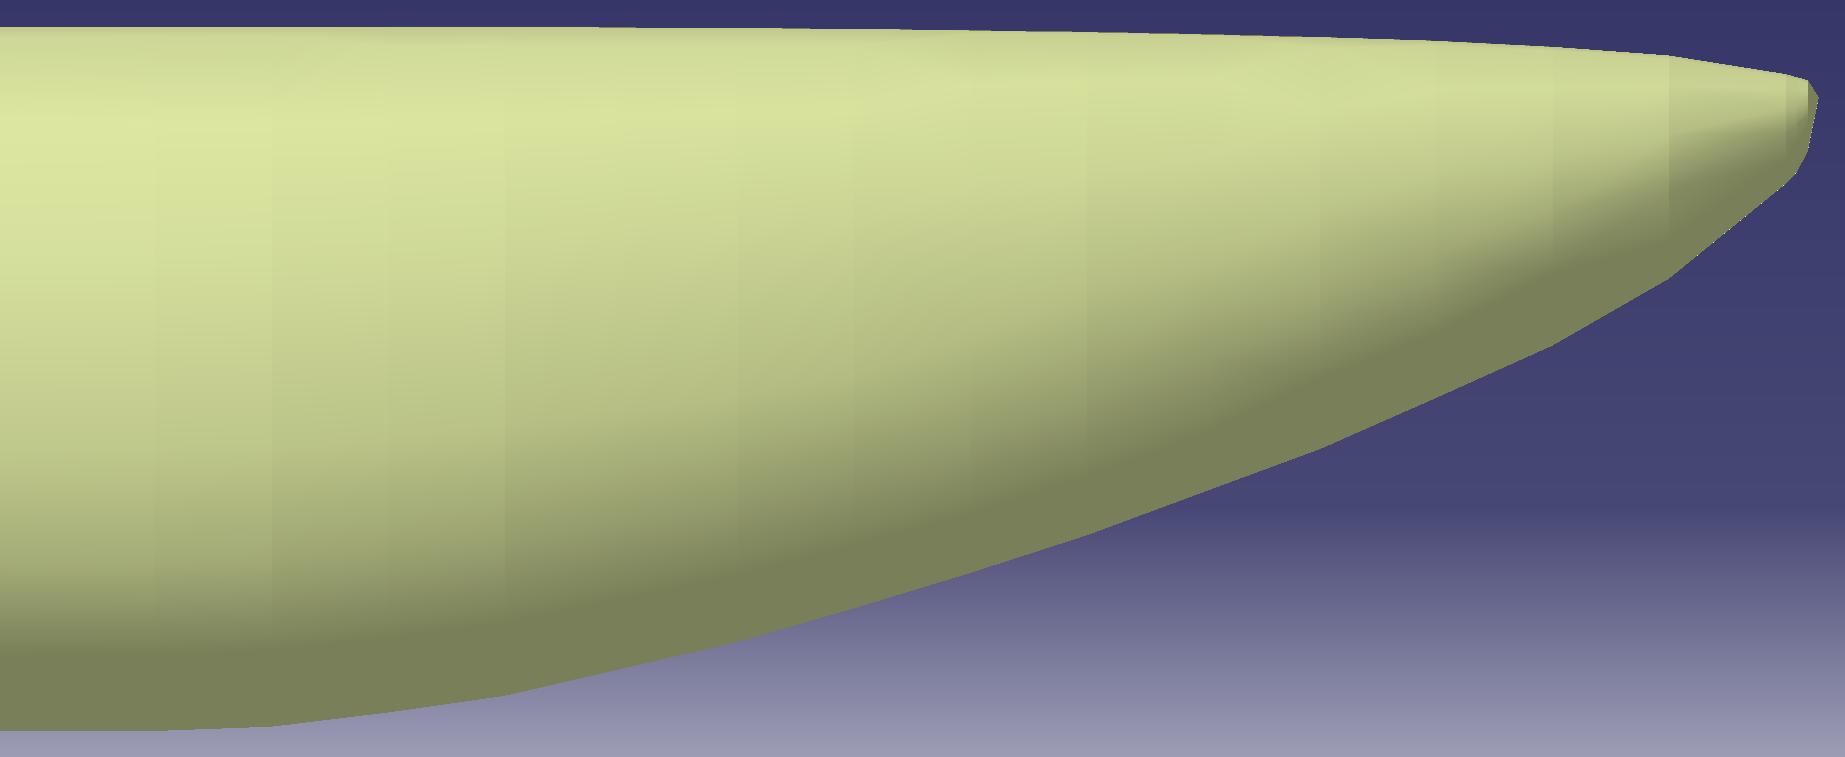
\includegraphics[width=6 cm]{Immagini/gui/CADfuselageTailOK.png}
		\caption{A detail of the tail of the fuselage obtained sewing together its parts.}
		\label{fig:goodTail}
\end{figure}


	\begin{figure}[H]
	\centering
		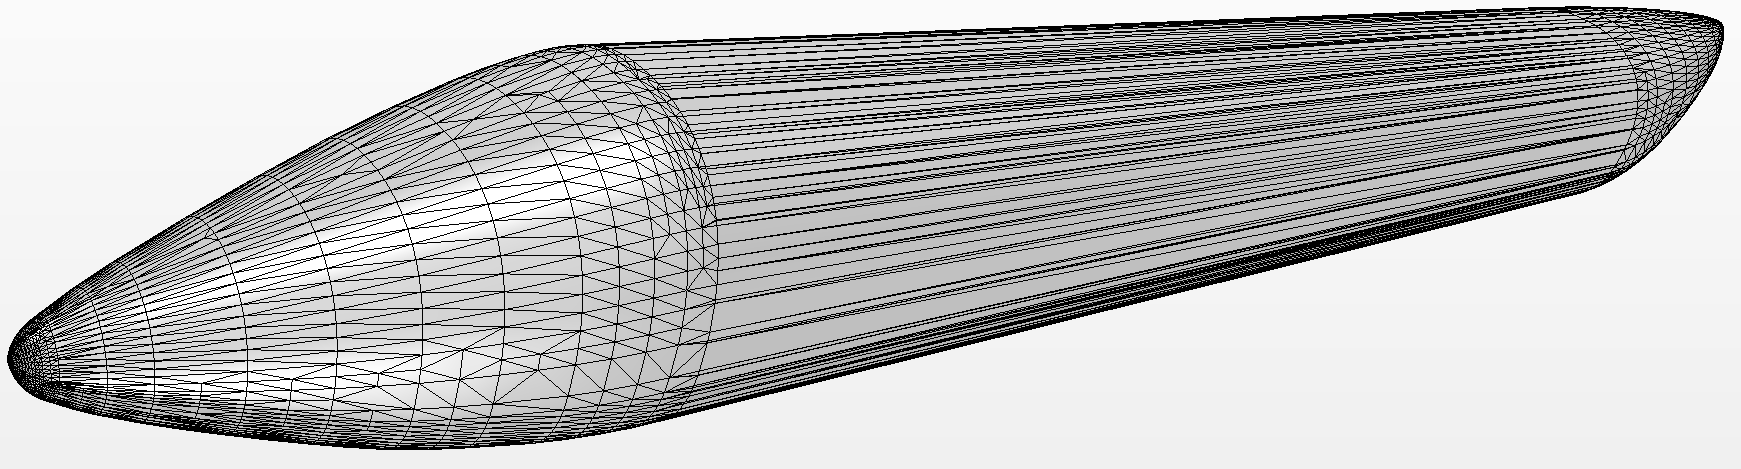
\includegraphics[width=12 cm]{Immagini/gui/CADfuselage}
		\caption{External fuselage shape exported as STEP file.}
		\label{fig:goodTail}
\end{figure}


\subsection{Interface with external software}
With ADOpT it's also possible to execute some high-fidelity analyses using external tools (i.e. CFD Navier-Stokes solver, panel method, FEM for structural static and dynamic analysis, etc.) by importing the dedicated output (such as a CAD model) produced by the software. The higher-fidelity tools could improve the results obtained and give therefore some useful clues in order to start a new design loop with different requirements and/or different constraints. The possibility to interface the software with drawings and graphical representation (i.e. CAD or Catia) of the designed aircraft is also very important.

\begin{figure}[H]
	\centering
		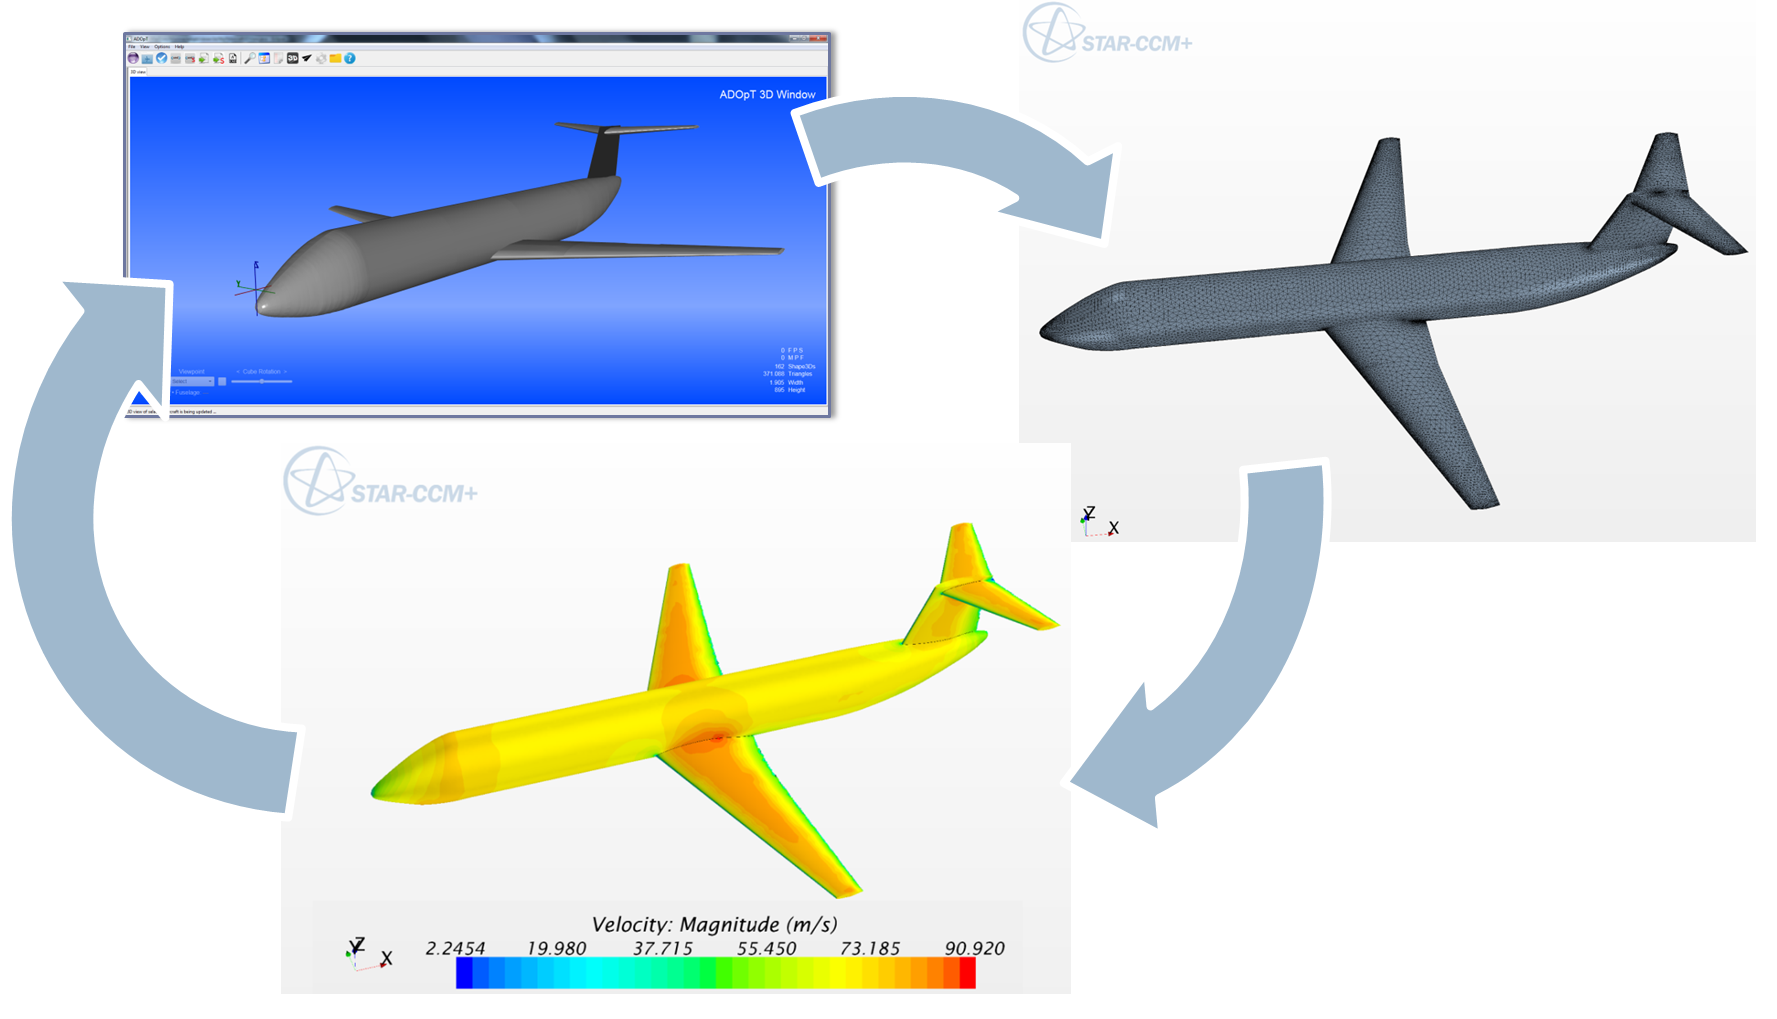
\includegraphics[width=12.9 cm]{Immagini/interface}
		\caption{Interface with external CFD tools.}
		\label{fig:badTail}
	\end{figure}
	
\section{In Development}

JPAD library is currently being developed in order to achieve a complete analysis of an aircraft and its optimization. The development is actually moving on a complete reorganization of the input file, and the implementation of other methods of analysis. Anyway, to date, it was reached an advanced level of implemented methods and a full functionality of some modules.

\subsection{Input File}

In order to obtain an useful and intuitive input structure a new data arrangement is in development. The JPAD input files are actually in XML data format. This extension will not change, but the purpose of the new structure is to allow the user to easily manage the input data in order to execute the desired analyzes.\\
The structure is inspired by that proposed by SUAVE. SUAVE is an open source suite constructed as a modular set of analysis tools written in Python and it is currently being developed in the Aerospace Design Lab at Stanford University. \cite{suave}
%This tool is based on a three input data structure as in the following figures.

\begin{figure}[H]
\centering
	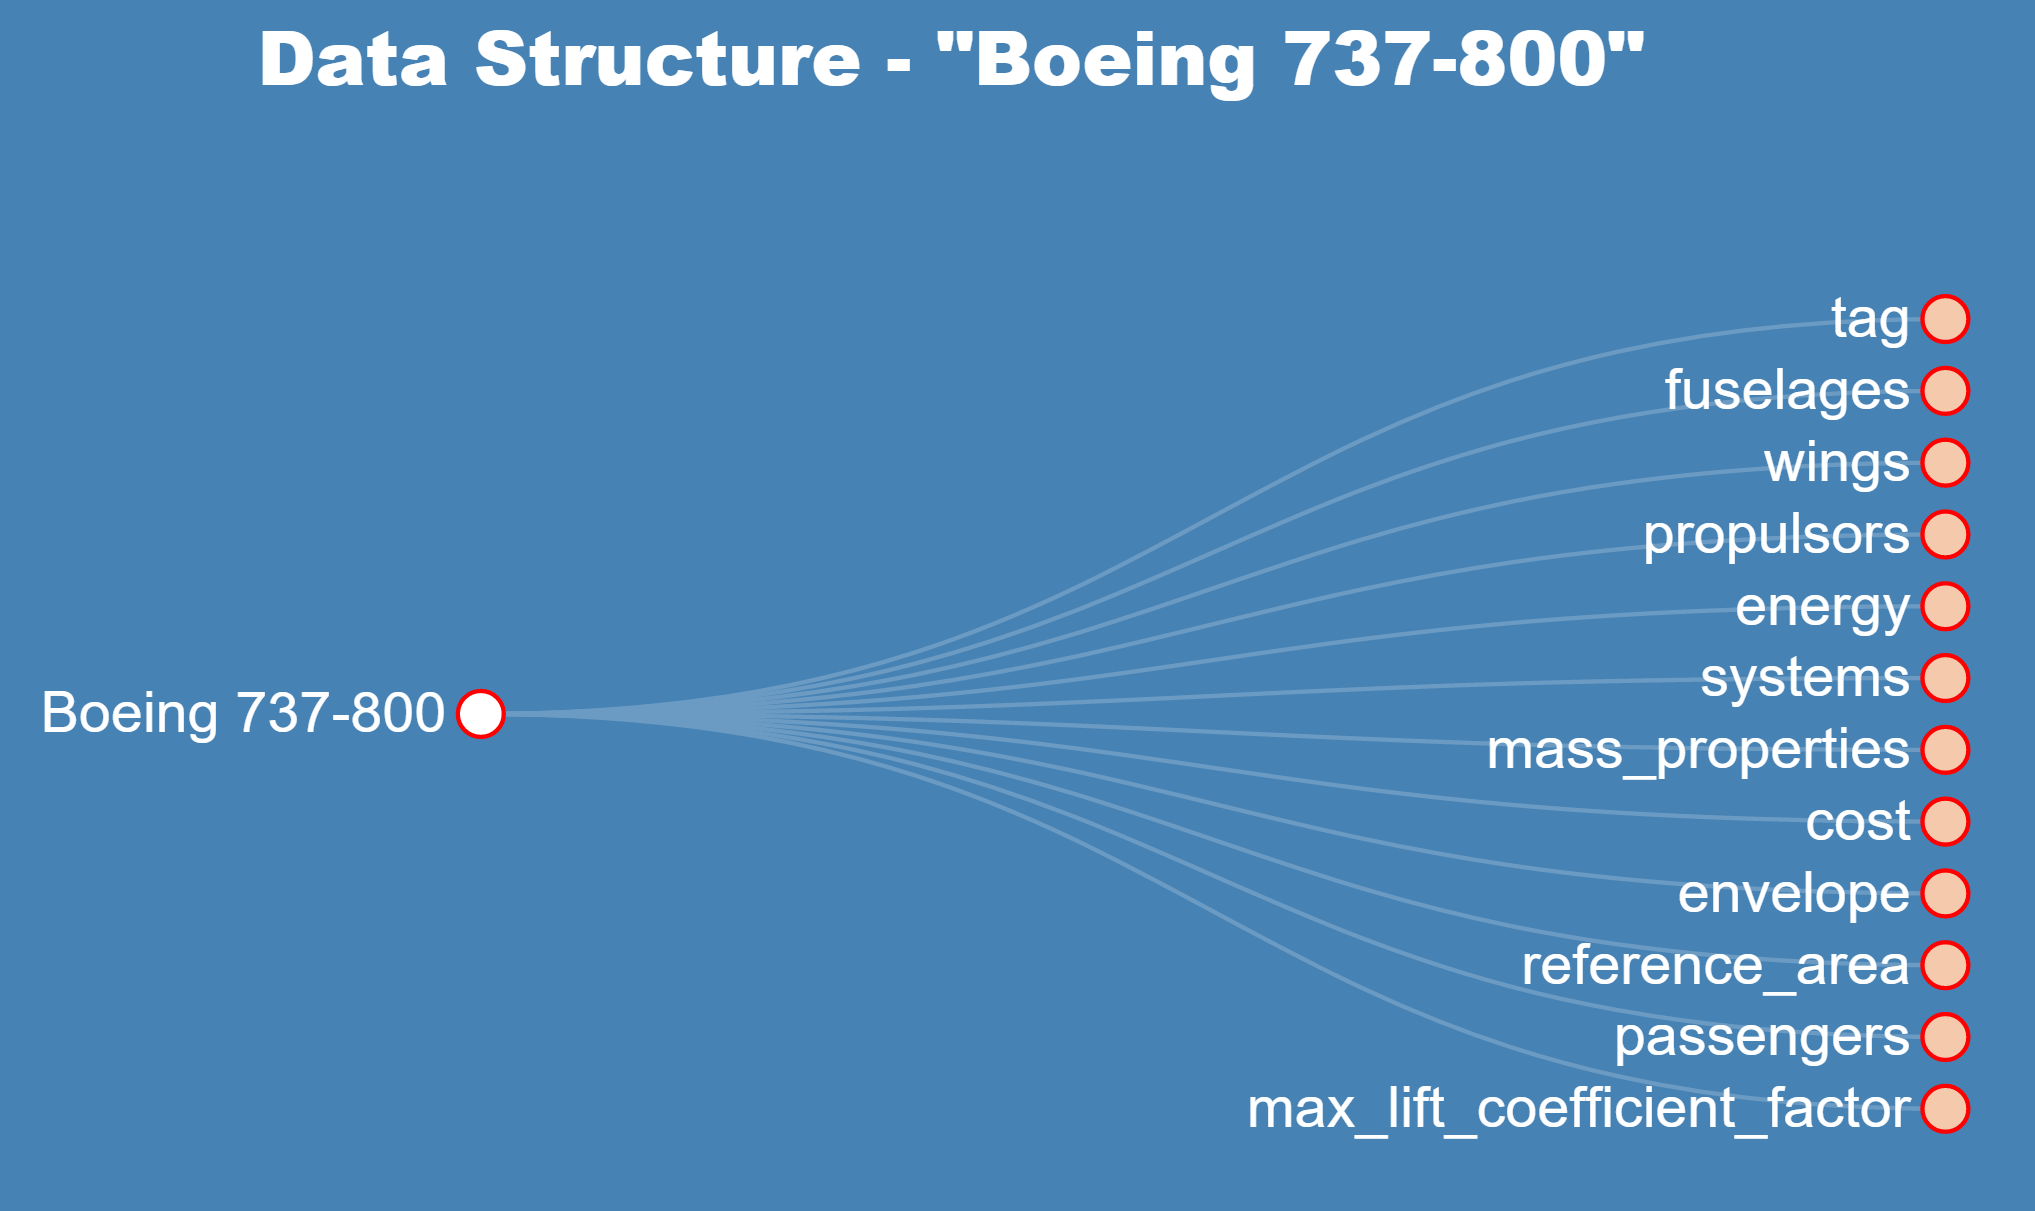
\includegraphics[width=11cm]{Immagini/suave/flowchartBoeing1}
	\caption{Data Structure used by SUAVE.}
	\label{fig:suave1}
\end{figure}

%
%\begin{figure}[H]
%	\centering
%	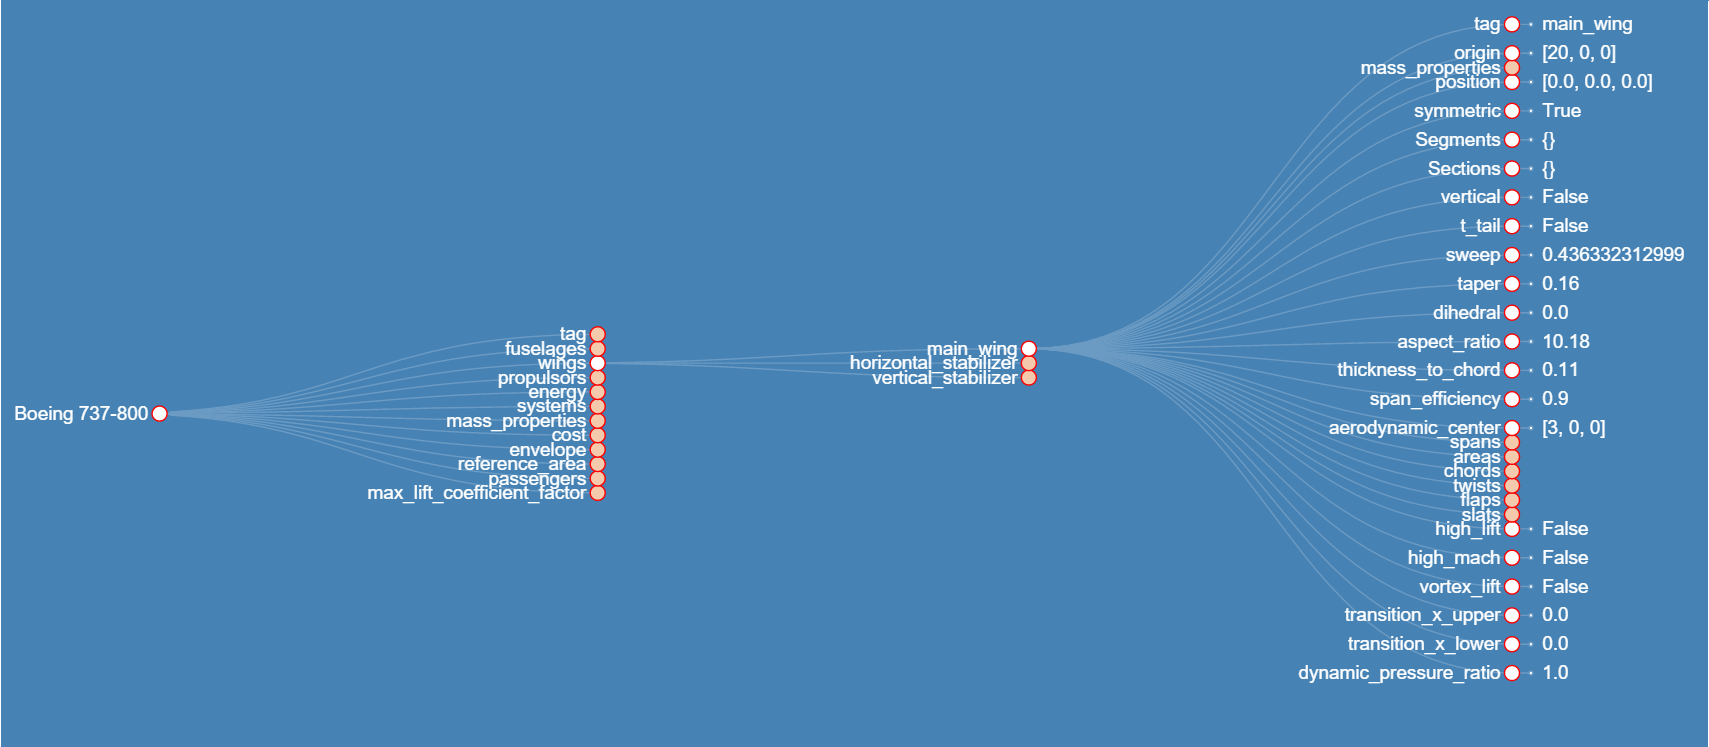
\includegraphics[width=12 cm]{Immagini/suave/flowchartBoeing2}
%	\caption{Data Structure used by SUAVE.}
%	\label{fig:suave2}
%\end{figure}



\begin{figure}[H]
\centering
	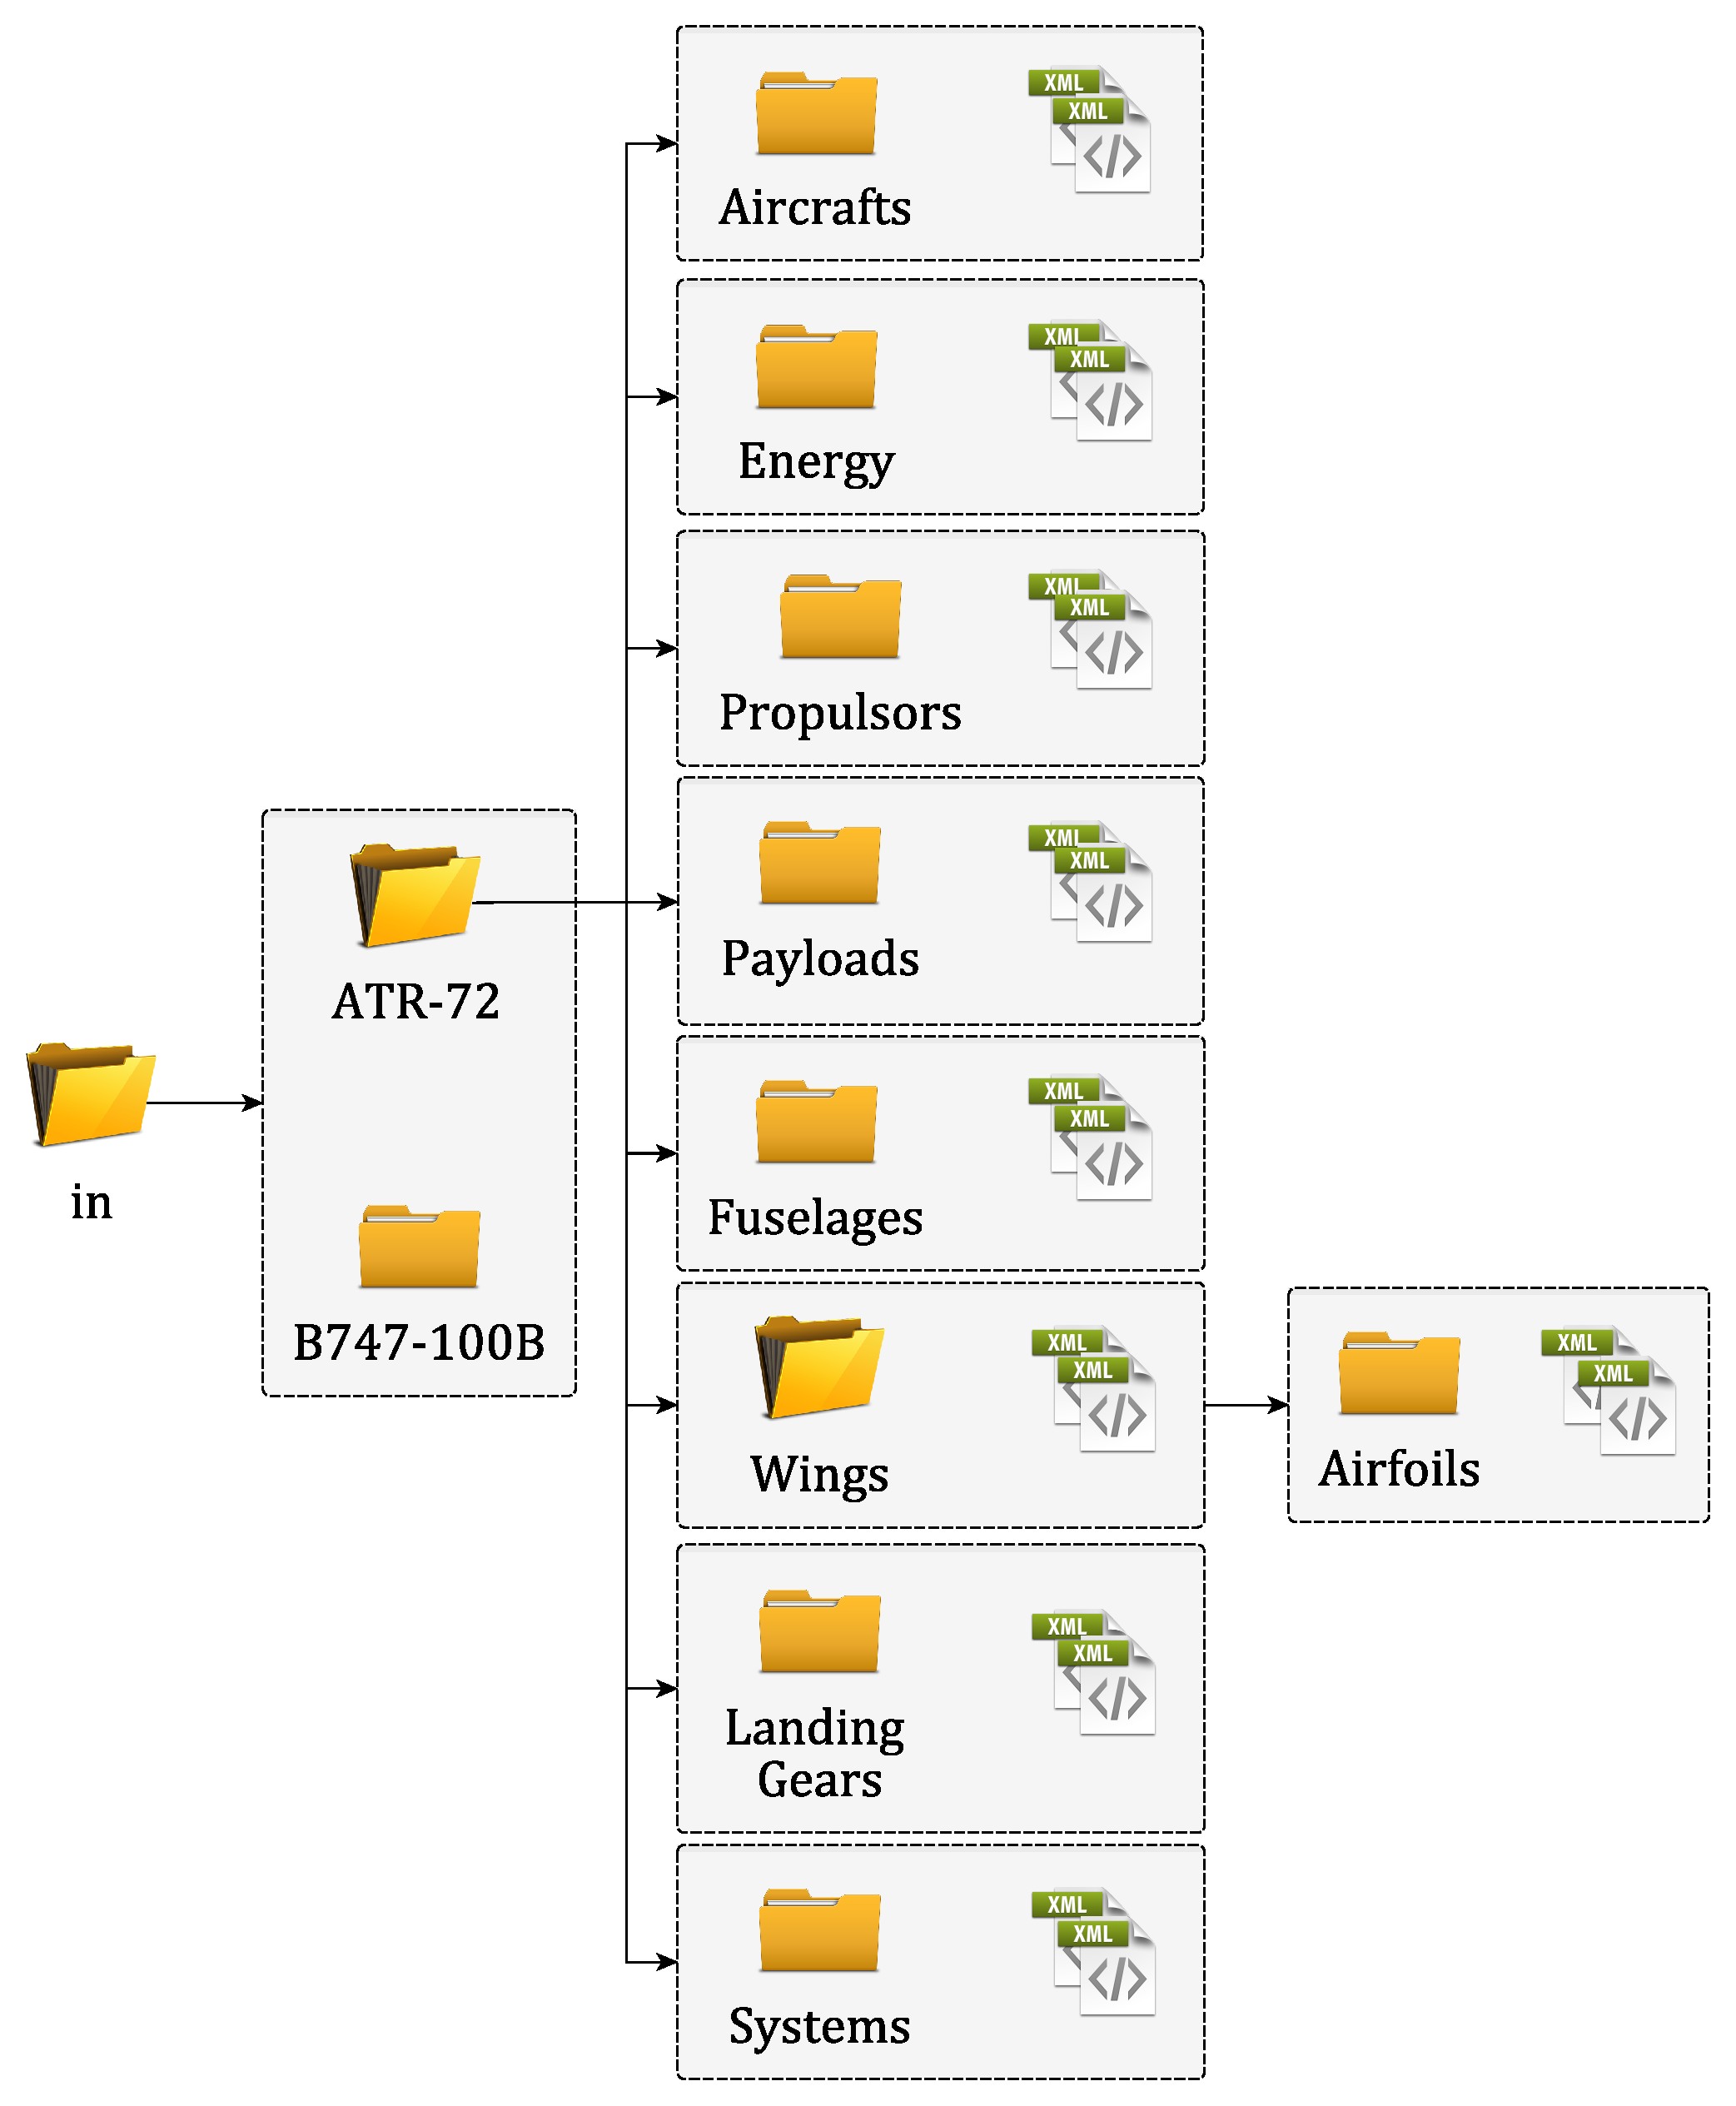
\includegraphics[width=11 cm]{Immagini/suave/Folder_Tree}
		\caption{Folder Structure in development.}
		\label{fig:suave3}
\end{figure}

The fundamental criteria on which the construction is based are expressed following.\\
In the input file folder, there are many sub-folder for different aircraft. In each of these there are several folders for component in which may be more XML file that corresponding to a different configuration. In fact, there is an XML file for each configuration of each aircraft component ( fuselage, lifting surfaces etc. ).In this way it's possible to choose different configuration for the same aircraft simply changing one or more XML input file.\\
 For the analysis the useful data will be explained in a user guide. User could make a complete analysis on a new aircraft, simply defining the required data and organize them in separated xml file. \\
 The main XML file is ``aircraft.xml'' which calls the other XML of the aircraft components. A typical file structure is in the following listings.
 
\begin{lstlisting}[frame=rbl,style=MyxmlStyle, caption={{\footnotesize XML input file for an aircraft.}},label= [style=\bfseries]{Listing}]
<?xml version="1.0" encoding="utf-8"?>
<jpad_config>
    <aircraft>
        <wings>
            <wing type="WING" file="wing.xml">
                <position>
                    <x unit="m">12.0</x>
                    <y unit="m"> 0.0</y>
                    <z unit="m"> 2.0</z>
                </position>
                <rigging_angle unit="deg">2.0</rigging_angle>
            </wing>
            <wing type="HTAIL" file="htail.xml">
                <position>
                    <x unit="m">30.0</x>
                    <y unit="m"> 0.0</y>
                    <z unit="m"> 4.0</z>
                </position>
                <rigging_angle unit="deg">0.0</rigging_angle>
            </wing>
            <wing type="VTAIL" file="vtail.xml">
                <position>
                    <x unit="m">30.0</x>
                    <y unit="m"> 0.0</y>
                    <z unit="m"> 5.0</z>
                </position>
                <rigging_angle unit="deg">0.0</rigging_angle>
            </wing>
        </wings>
        <fuselages>
            <fuselage file="fuselage.xml">
                <position>
                    <x unit="m">0.0</x>
                    <y unit="m">0.0</y>
                    <z unit="m">0.0</z>
                </position>
            </fuselage>
        </fuselages>
        <propulsors>
            <propulsor file="propulsor.xml">
                <position>
                    <x unit="m">12.0</x>
                    <y unit="m"> 5.0</y>
                    <z unit="m"> 0.0</z>
                </position>
                <tilting_angle unit="deg">2.0</tilting_angle>
                <yawing_angle unit="deg">0.0</yawing_angle>
            </propulsor>
            <propulsor file="propulsor.xml">
                <position>
                    <x unit="m">12.0</x>
                    <y unit="m">-5.0</y>
                    <z unit="m"> 0.0</z>
                </position>
                <tilting_angle unit="deg">2.0</tilting_angle>
                <yawing_angle unit="deg">0.0</yawing_angle>
            </propulsor>
        </propulsors>
    </aircraft>
</jpad_config>
\end{lstlisting}

\begin{lstlisting}[frame=rbl,style=MyxmlStyle, caption={{\footnotesize XML input file for an aircraft.}},label= [style=\bfseries]{Listing}]
<?xml version="1.0" encoding="utf-8"?>
<jpad_config>
    <wing mirrored="TRUE">
        <panels>
            <panel id="Inner panel">
                <semispan unit="m">4.0</semispan>
                <dihedral unit="deg">1.5</dihedral>
                <inner_section>
                    <airfoil file="naca63209.xml"/>
                    <geometric_twist unit="deg">0.0</geometric_twist>
                </inner_section>
                <outer_section>
                    <airfoil file="naca63209.xml"/>
                    <geometric_twist unit="deg">0.0</geometric_twist>
                </outer_section>
            </panel>
            <panel id="Outer panel" linked_to="Inner panel">
                <semispan unit="m">7.0</semispan>
                <dihedral unit="deg">3.5</dihedral>
                <outer_section>
                    <airfoil file="naca63209.xml"/>
                    <geometric_twist unit="deg">-2.5</geometric_twist>
                </outer_section>
            </panel>
        </panels>
        <symmetric_flaps>
            <symmetric_flap id="Inner flap" type="SINGLE_SLOTTED">
                <inner_station_spanwise_position type="PERCENT_SEMISPAN" ref_to="FULL_SEMISPAN">
                    <value>0.15<value/>
                </inner_station_spanwise_position>
                <outer_station_spanwise_position type="PERCENT_SEMISPAN" ref_to="FULL_SEMISPAN">
                    <value>0.45<value/>
                </outer_station_spanwise_position>
                <percent_chord value="40"/>
                <angle_range unit="deg">[0.0,40.0]</angle_range>
            </symmetric_flap>
        </symmetric_flaps>
        <slats>
            <slat linked_to="Inner flap" type="SINGLE">
                <percent_chord value="10"/>
                <angle_range unit="deg">[0.0,10.0]</angle_range>
            </slat>
        </slats>
        <asymmetric_flaps>
            <asymmetric_flap id="Aileron" type="PLAIN">
                <inner_station_spanwise_position type="PERCENT_SEMISPAN" ref_to=
                                                                                                "FULL_SEMISPAN">
                    <value>0.75<value/>
                </inner_station_spanwise_position>
                <outer_station_spanwise_position type="PERCENT_SEMISPAN" ref_to=
                                                                                                 "FULL_SEMISPAN">
                    <value>0.97<value/>
                </outer_station_spanwise_position>
                <percent_chord value="20"/>
                <angle_range unit="deg">[-5.0,10.0]</angle_range>
                <differential_deflection_factor value="1.0"/>
            </asymmetric_flap>
        </asymmetric_flaps>
    </wing>
</jpad_config>
\end{lstlisting}

\subsection{Calculation modules}
Currently the software is able to esimate the aircraft weight breakdown, the center of gravity location, calculate some aerodynamic parameters and estimate the performance. All these types of estimates can be usually performed using several analysis methods, comparable and interchangeable. 
It is also provided a static longitudinal stability analysis, take-off performances and the generation of Payload Range chart.\\
Future targets for the software are the implementation of landing performances, ultimate the directional static stability % ... 


\subsection{Optimization Process}
It has always been the engineer’s dream to have all aspects of analysis done in a relatively short time period so that many different configurations can be examined and the best suitable product can be delivered on time. Although this may still be a dream, actual design turn-around time has become shorter due to the use of mathematical optimization techniques which have been
introduced into the design process.\cite{torenbeek2013advanced}
As all analysis modules inside the JPADCore package will be completed and tested, the final purpose of the code will be to allow users to define a certain numbers of macroscopical geometrical parameters, along with a given objective function, and to receive as output the best set of the previous parameters which suits the wanted objective.
